\documentclass[notitlepage, reprint, nofootinbib]{revtex4-1}
\usepackage[utf8]{inputenc}

% Mathematics and symbols:
\usepackage{amsmath, gensymb, amsthm, physics, mhchem}
% Figures:
\usepackage{tikz, graphicx}
\usepackage[caption=false]{subfig}

% Other:
\usepackage{hyperref}

\hypersetup{
    colorlinks=true,
    linkcolor=orange,
    filecolor=magenta,      
    urlcolor=orange,
}

\usepackage{algorithm}
\usepackage{algpseudocode}


% Document formatting 
\setlength{\parskip}{1mm}
\setlength{\parindent}{0mm}


%\renewcommand{\thesubsubsection}{\alph{subsubsection})}


\begin{document}
\title{FYS3150 - Project 3}
\author{Frida Larsen}

% Abstract
\begin{abstract}
This report investigates four approaches to numerical integration. Two deterministic approaches using Gaussian quadrature and two probabilistic approaches using Monte Carlo integration. The methods are compared in terms of both accuracy and efficiency. Although all of the methods converge towards the analytical result, the Monte Carlo based methods are generally more efficient than the Gaussian quadrature based methods. Our Gaussian quadrature methods used Legendre polynomials and a mixture of Legendre and Laguerre polynomials. The mixed method turned out to be the most accurate, although pure Gauss-Legendre was slightly faster. One of the Monte Carlo methods used importance sampling, which significantly improved the convergence rate, although it was slightly slower. Surprisingly, a parallelisation of the importance sampling algorithm turned out to be the slowest of the Monte Carlo methods. It is unclear whether this is due to our implementation or our hardware, which shows how important it is to be consistent with how algorithms are timed. 
\end{abstract}

\maketitle

\section{Introduction}
Integration is a very important concept in mathematics. Solving convoluted integrals can be both tricky and time-consuming, not to mention impossible in some cases. For this reason it is important to have reliable tools for solving integrals numerically.\\[2mm]
The aim of this project is to implement and investigate the accuracy and efficiency of two approaches for numerical approximation of integrals, namely Gaussian quadrature and Monte Carlo methods. The approaches will be compared to each other in their ability to accurately solve a six-dimensional integral with quantum mechanics applications.\\[2mm]
All relevant code may be found in the GitHub repository 'FYS3150-Computational-Physics'\footnote{\href{GitHub Repository}{https://github.com/fridalarsen/FYS3150-Computational-Physics}} under the Project3 folder. This folder also includes a Figures folder, which holds all the figures presented in this text. The main framework of this project is written as a class which may be found in the '\texttt{project3.py}'-program.
\section{Theory - Quantum Mechanics}
\subsection{The Helium Atom}
A helium atom contains two electrons. For this project, we will model the wave function of each electron as the single-particle wave function of an electron in the hydrogen atom. For such an electron i in the 1s state we have the wave function 
$$\psi_{1s}(\vb{r}_i)=e^{-\alpha r_i}, $$
where $\alpha$ is a parameter corresponding to the charge of the atom and 
$$\vb{r}_i=x_i\vb{e}_x+y_i\vb{e}_y+z_i\vb{e_z}, \quad r_i=\sqrt{x_i^2+y_i^2+z_i^2}.$$ 
Combining the wave functions of two such electrons yields 
$$\Psi(\vb{r}_1,\vb{r}_2) = e^{-\alpha(r_1+r_2)}.$$
As the charge of the helium atom is 2, we set $\alpha=2$. The expectation value of the correlation energy between two electrons that repel each other via the Coulomb interaction is given by 
\begin{equation}\label{int}I=\expval{\frac{1}{|\vb{r}_1-\vb{r}_2|}}=\int_{-\infty}^{\infty}\dd \vb{r}_1\dd \vb{r}_2 e^{-2\alpha(r_1+r_2)}\frac{1}{|\vb{r}_1-\vb{r}_2|}.\end{equation} 
The closed form answer of this integral is
\begin{equation}\label{int_ans}\expval{\frac{1}{|\vb{r}_1-\vb{r}_2|}}=\frac{5\pi^2}{16^2}.\end{equation}
The integral of equation \ref{int} can also be expressed in terms of spherical coordinates, 
\begin{align}
	I=\int_0^\infty r_1^2\dd r_1\int_0^\infty r_2^2\dd r_2 \int_0^\pi \dd\cos(\theta_1)\int_0^\pi\dd\cos(\theta_2)\nonumber\\
	\int_0^{2\pi}\dd\phi_1\int_0^{2\pi}\dd\phi_2\frac{e^{-2\alpha(r1+r2)}}{r_12},\label{spheric_int}
\end{align}
where 
$$\frac{1}{r_{12}}=\frac{1}{\sqrt{r_1^2 + r_2^2 -2r_1r_2\cos(\beta)}}$$
and 
$$\cos(\beta)=\cos(\theta_1)\cos(\theta_2)+\sin(\theta_1)\sin(\theta_2)\cos(\phi_1-\phi_2).$$
\newpage
\section{Theory - Numerical Integration}
The goal of numerical integration is to approximate the value of a definite integral to a given degree of accuracy. There are many methods that can be used for this purpose. In this project we will focus on two families of numerical integration methods, namely Gaussian Quadrature and Monte Carlo methods.\\[2mm]
The basic idea of numerical integration is to estimate an integral by 
\begin{equation}\label{numint}I=\int_a^bf(x)\dd x \approx \sum_{i=1}^N\omega_i f(x_i),\end{equation}
where $\omega_i$ are weights and $x_i$ are the mesh points. In the case that the integrand $f(x)$ is not smooth, we can render it smooth by extracting a weight function $W(x)$ in the following way:
\begin{equation}\label{numint_smooth}I=\int_a^bf(x)\dd x=\int_a^bW(x)g(x)\dd x\approx \sum_{i=1}^N \omega_i g(x_i).\end{equation}
Extracting a weight function in this way may of course also be done for a smooth function.

\subsection{Gaussian Quadrature}
A Gaussian quadrature formula integrates all polynomials of degree $2N-1$ exactly with $N$ distinct quadrature points, that is 
\begin{equation}\label{gq1}\int_a^bW(x)P_{2N-1}\dd x=\sum_{i=1}^N\omega_iP_{2N-1}(x_i)\end{equation}
exactly. We must then approximate $g(x)$ from equation \ref{numint_smooth} by a polynomial. In summary, Gaussian quadrature works as follows: 
\begin{equation}\label{gq2}\int_{-1}^1 f(x)\dd x\approx\int_{-1}^1 W(x)P_{2N-1}(x)\dd x =\sum_{i=0}^{N-1} P_{2N-1}(x_i)\omega_i.\end{equation}
The fact that only $N-1$ points are needed in Gaussian quadrature results from rewriting the polynomial in terms of orthogonal polynomials\cite{lecture_notes}. What orthogonal polynomials to use depends on the weight function.  \\[2mm]
The mesh points and the weights are then determined by the zeros of the relevant orthogonal polynomial and elements of a matrix also defined by the orthogonal polynomial. 
\newpage
\subsubsection{Gauss-Legendre}
When the weight function $W(x)=1$ and integral limits are $[-1,1)$, the Legendre polynomials may be used. The Legendre polynomials are given by the Rodrigues' type formula: 
\begin{equation}\label{rodrigues1}L_n(x)=\frac{1}{2^n n!}\dv[2]{x} (x^2-1)^n.\end{equation}
They can also be calculated recursively by 
\begin{equation}\label{legendre} L_{j+1} = \frac{(2j+1)xL_j-jL_{j-1}}{j+1}.\end{equation}
The derivative is given by
\begin{equation}\label{ddlegendre} \dv{x} L_j = \frac{j (xL_j-L_{j-1})}{x^2-1}.\end{equation}
The zeros of the Legendre polynomials can be organised into a matrix: 
\begin{equation}\label{L_hat}\hat{L}=\mqty(L_0(x_0)&L_1(x_0)&\cdots&L_{N-1}(x_0)\\L_0(x_1)&L_1(x_1)&\cdots&L_{N-1}(x_1)\\ \cdots &\cdots&\cdots&\cdots\\L_0(x_{N-1})&L_1(x_{N-1})&\cdots&L_{N-1}(x_{N-1})),\end{equation}
so that 
\begin{equation}\label{omega_leg}\omega_i =(\hat{L}^{-1})_{0i}.\end{equation}

\subsubsection{Gauss-Laguerre}
When the weight function is $W(x)=x^\alpha e^{-x}$ and the integral limits are $[0,\infty)$ the Laguerre polynomials may be used. The Laguerre polynomials are given by the Rodrigues' type formula
\begin{equation}\label{rodrigues2}\mathcal{L}_n(x)=\frac{1}{n!}\Big(\dv{x}-1\Big)^nx^n.\end{equation}

\subsection{Monte Carlo}
Monte Carlo integration is inherently different from Gaussian quadrature in that it is not deterministic, but rather based on random numbers.\\[2mm]
The average value of a function $f$ is given by
$$\expval {f}=\int_{-\infty}^\infty \dd x\ p(x) f(x),$$
where $p(x)$ is a probability distribution function (PDF). What PDF is used will depend on the problem. The basic idea of Monte Carlo is to add such a probability function to the integral;
\begin{align}
	\int_a^b f(x) \dd x&=\int_a^b \dd x\ p(x) \frac{f(x)}{p(x)}\nonumber \\
	&\approx \frac{1}{N}\sum_{i=1}^{N} \frac{f(x_i)}{p(x_i)}, \label{MC_formula}
\end{align}
where the numbers $x_i$ are drawn from the specified PDF and $N$ is the number of Monte Carlo samples (number of x-values drawn). The law of large numbers ensures that we get closer to the exact value of the integral as $N$ increases. Specifically, the standard error, $\sigma/\sqrt{N}$, of the integral approaches 0. The variance is given by
\begin{equation}\label{var}\sigma^2_f = (\expval{f^2} - \expval{f}^2)=\sum_{i=1}^N (f(x_i)-\expval{f})^2p(x_i).\end{equation}
An important concept in Monte Carlo integration is that of importance sampling. The idea is to choose a PDF which has the general shape of the integrand. 
\begin{figure}[h!]
	\centering
	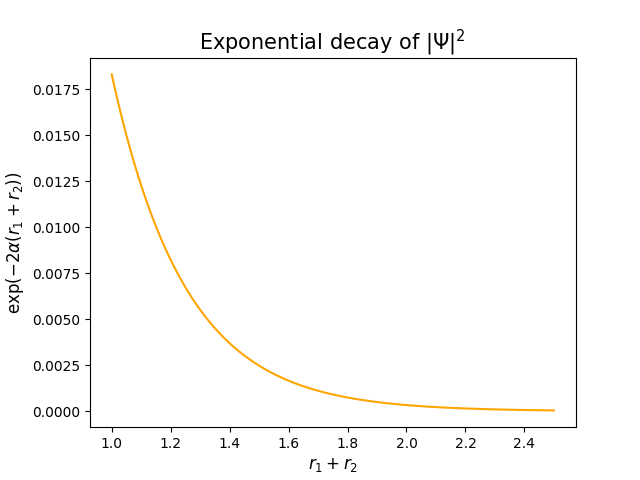
\includegraphics[width=0.5\textwidth]{../Figures/wavefunc.png}
	\caption{Exponential decay of the integrand of equation \ref{int}.}
	\label{wavefunc}
\end{figure}
\section{Method}
\subsection{Gaussian Quadrature}
\subsubsection{Gauss-Legendre}\label{GLeg}
The first obstacle for using Gauss-Legendre quadrature in order to determine the integral of equation \ref{int}, is the interval of integrations. Not only is the integral supposed to be taken from $-\infty$ to $+\infty$, but Gauss-Legendre only permits integrals from -1 to 1.\\[2mm]
For large $r_1$s and $r_2$s, the fraction $\frac{1}{|\vb{r}_1-\vb{r}_2|}$ becomes small, as it is highly unlikely that the two electrons will meet. Thus, the exponential will dominate. The radius, $r_i$, cannot be negative. The exponential part of the integrand is plotted in figure \ref{wavefunc}. From this figure we see that the integrand becomes 0 at roughly $(r_1+r_2)=2.2$, so there is no point in integrating further than this. Thus, we can approximate 
$$\int_{-\infty}^{+\infty}\rightarrow \int_{-2.2}^{2.2}.$$
It remains to transform these new limits into the Gauss-Legendre approved integral limits. We do this by changing the variable of integration so that
$$\int_a^b f(t)\dd t= \frac{b-a}{2}\int_{-1}^1 f\big(\frac{b-a}{2}x+\frac{b+a}{2}\big)\dd x.$$
The next step is to find the mesh points $x_k$, which are the Legendre zeros, and the corresponding weights $\omega_k$. The mesh points can then be transformed back to the original interval by 
\begin{equation}\label{transint}t_k=\frac{b+a}{2}+x_k\frac{b-a}{2}.\end{equation}
The original integral may now be approximated by 
\begin{equation}\label{int5}\int_a^bf(t)\dd t \approx \sum_{k=0}^{N-1}\omega_k f(t_k).\end{equation}
Gauss-Legendre quadrature for solving an integral is summarised in the following algorithm:
\begin{algorithm}[H]
	\caption{Gauss-Legendre quadrature for approximating an integral.}
	\begin{algorithmic}[1]
		\State Find mesh points and weights using the zeros of $L_N$ and equation \ref{omega_leg}. 
		\State Transform mesh points back to original interval by equation \ref{transint}. 
		\State Compute the integral through equation \ref{int5}.
	\end{algorithmic}
\end{algorithm}
Our goal is to approximate the integral in equation \ref{int}. In order to extend out methods to n-dimensional integrals, we would need to compute the sum 
\begin{align}
	&\int_a^b \cdots \int_c^d f(t_1,t_2,\ldots,t_n)\dd t_1 \cdots \dd t_n \nonumber\\
	&\approx\sum_{i=0}^{N-1} \cdots \sum_{j=0}^{N-1} \omega_i\cdots \omega_j f(t_i, \ldots, t_j). \label{bigint5}
\end{align}
However, the method for finding the mesh points and the weights only depend on N, not on a and b. In our case
$$f(t_i,\ldots,t_j) = |\Psi(\vb{r}_1, \vb{r}_2)|^2=e^{-2\alpha(r_1+r_2)}\frac{1}{|\vb{r}_1-\vb{r}_2|}.$$ 
\newpage
Thus, we have the following algorithm: 
\begin{algorithm}[H]
	\caption{Gauss-Legendre quadrature for approximating the integral of equation \ref{int}.}
	\begin{algorithmic}[1]
		\State Find mesh points and weights using the zeros of $L_N$ and equation \ref{omega_leg}. 
		\State Transform mesh points back to original interval for each dimension by equation \ref{transint}. 
		\State Compute the integral through equation \ref{bigint5}.
	\end{algorithmic}
\end{algorithm}

\subsubsection{Mixed Gaussian quadrature: Legendre and Laguerre}
The basis for Gauss-Laguerre is essentially the same as Gauss-Legendre. As before, we begin by assessing the integration interval. Gauss-Laguerre may be used for integrals from 0 to $\infty$.\\[2mm]
We observe that the integral $I$ written in spherical coordinates (equation \ref{spheric_int}) contains two such integrals (the radial components). For the remaining 4 angular integrals, we will continue to use Gauss-Legendre. The procedure is essentially the same as before, except that we now need to extract the weight function from the integrand. The resulting integrand is then 
$$f(r_1, r_2, \theta_1, \theta_2, \phi_1, \phi_2) = \sin(\theta_1)\sin(\theta_2)\frac{e^{-3(r_1+r_2)}}{r_{12}},$$
where we have inserted $\alpha=2$ and $r_{12}$ is defined as before.\\[2mm]
In order to find the Gauss-Laguerre weights and mesh points, we will use the program \texttt{gauss\_laguerre.cpp}\cite{gauss-laguerre}.

\subsection{Monte Carlo Integration}
The integral we wish to solve is six-dimensional. We must then implement the formula \ref{MC_formula} for each of these dimensions. Thus we have
\begin{align}
	\int_{a_1}^{b_1}\dd x_1 &\dots \int_{a_n}^{b_n} \dd x_n \ f(x_1, \ldots, x_n)\nonumber\\
	&=\int_{a_1}^{b_1}\dd x_1 \dots \int_{a_n}^{b_n} \dd x_n\ p(x_1,\ldots,x_n)\frac{f(x_1,\ldots, x_n)}{p(x_1,\ldots,x_n)}\nonumber\\
	&\approx \frac{1}{N} \sum_{i=1}^N \frac{f(x_{1,i},\ldots,x_{n,i})}{p(x_{1,i},\ldots,x_{n,i})}.\label{MC_ndim}
\end{align}
In the case that the $x$'s are independent of each other, we can factorise 
$$p(x_{1,i},\ldots, x_{n,i})=p(x_{1,i})\cdots p(x_{n,i}).$$
Thus, we have the following general Monte Carlo algorithm: 
\begin{algorithm}[H]
	\caption{Monte Carlo integration for approximating an $n$-dimensional integral.}
	\begin{algorithmic}[1]
		\State Choose number of samples, $N$.
		\State For each step in the sum, draw $n$ random numbers $x_{j,i}$ from the specified PDF.
		\State Evaluate $f(x_{1,i}, \ldots, x_{n,i})/p(x_{1,i},\ldots,x_{n,i})$.
		\State Divide sum by number of samples, per equation \ref{MC_ndim}.
	\end{algorithmic}
\end{algorithm}

\subsubsection{Uniform distribution}
We begin with the brute force method, using the integrand of equation \ref{int} and drawing samples from the uniform distribution. The uniform distribution is given by 
\begin{equation}\label{uni_dist}p(x)=\begin{cases} \frac{1}{z-w} \quad &\text{for $w \leq x \leq z$}\\ 0 \quad &\text{for $x < w$ or $x > z$.}\end{cases} \end{equation}
We need to choose $w$ and $z$ so that the integration limits lie within the interval $\qty[d, e]$. We use the same integration limits as in section \ref{GLeg}, and set these limits to also be the boundaries of the PDF. 

\subsubsection{Exponential distribution}\label{exp_distr}
For this method we will use the integrand of equation \ref{spheric_int}. Because our integrand has the general shape of an exponential function, we will use the exponential distribution for importance sampling. In general, the exponential distribution is given by
\begin{equation}\label{exp_dist} p(x)=\begin{cases}\lambda e^{-\lambda x} \quad  &\text{for $x\geq 0$}\\ 0\quad &\text{for $x<0$},\end{cases}\end{equation}
but we will set $\lambda=1$ for simplicity. 

\subsubsection{Parallelisation}
The final method we will investigate is that of parallelisation. In this case we will use the same method as in \ref{exp_distr}, but parallelise the code using MPI\cite{MPI}. 
\newpage
\begin{figure}[h!]
	\centering
	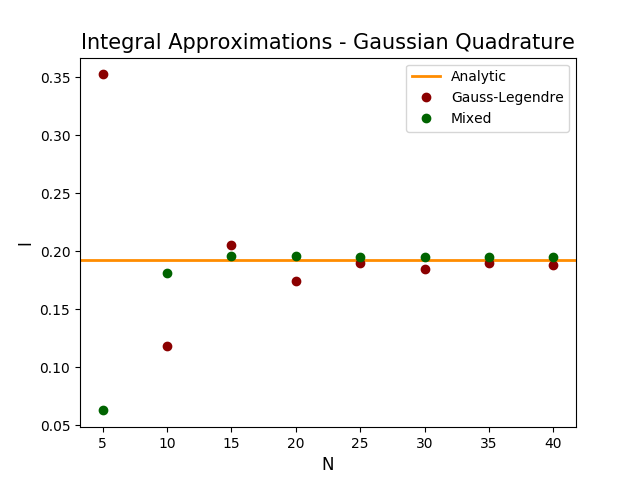
\includegraphics[width=0.45\textwidth]{../Figures/QC_quadrature.png}
	\caption{Integral values calculated with Gaussian quadrature compared to analytic solution. }
	\label{res1}
\end{figure}
\begin{figure}[h!]
	\centering
	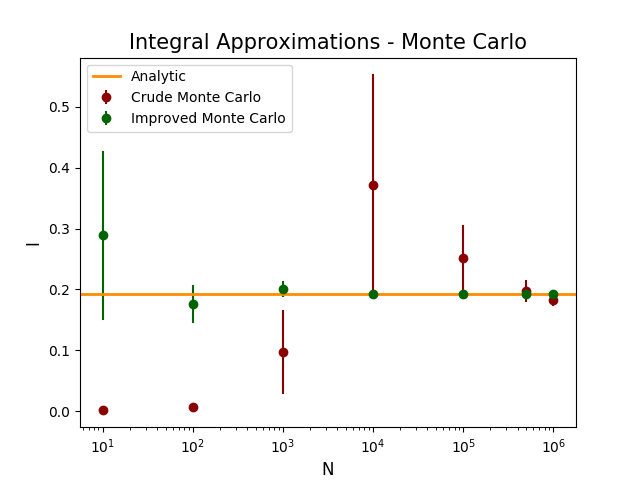
\includegraphics[width=0.45\textwidth]{../Figures/MC.png}
	\caption{Integral values calculated with Monte Carlo integration compared to analytic solution. The standard error is indicated as errorbars.}
	\label{res2}
\end{figure}
\section{Results}
The approximated integrals as computed with Gaussian quadrature and Monte Carlo integration are presented in figures \ref{res1} and \ref{res2} respectively. The latter also contains the standard error of each value as an errorbar.\\[2mm]
The time taken by each of the Gaussian quadrature algorithms and the Monte Carlo algorithms are plotted in figures \ref{res3} and \ref{res4}. The standard deviation of the timing-data is indicated in the Monte Carlo plot as errorbars. There was no point in indicating this in the Gaussian plots, as the standard deviation was too small to be visible next to the point indicators. \\[2mm]
Note that, due to hardware restrictions, only 2 processes were run in parallel for the parallelised Monte Carlo integration. 
\begin{figure}[h!]
	\centering
	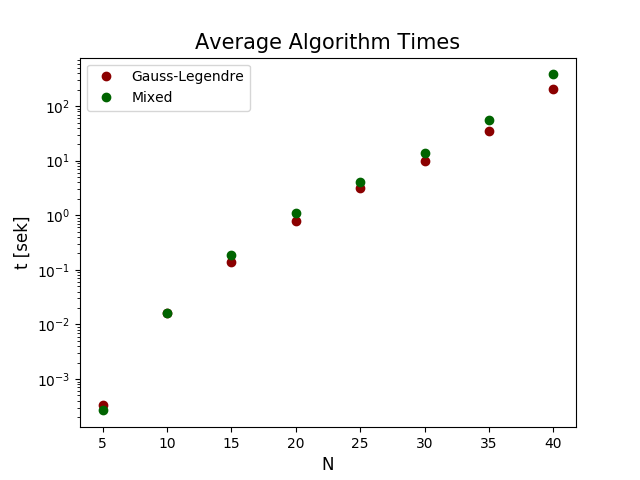
\includegraphics[width=0.45\textwidth]{../Figures/algo_times_GQ.png}
	\caption{Time measurements of Gaussian quadrature algorithms.}
	\label{res3}
\end{figure}
\begin{figure}[h!]
	\centering
	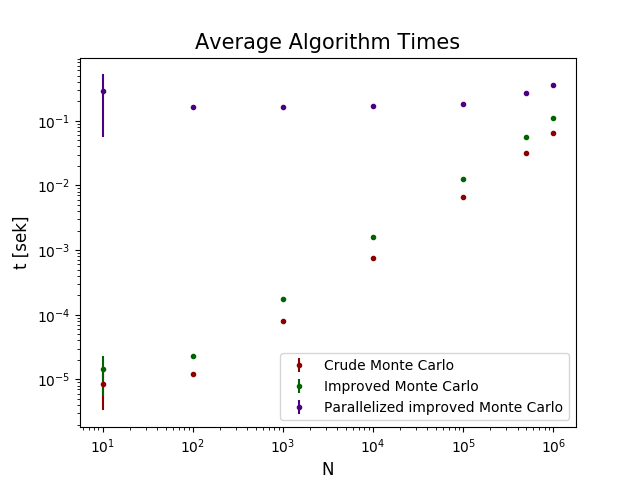
\includegraphics[width=0.45\textwidth]{../Figures/algo_time_MC.png}
	\caption{Time measurements of Monte Carlo algorithms. Standard deviation of measurements indicated as errorbars.}
	\label{res4}
\end{figure}
\section{Discussion}
From figure \ref{res1} we see that although both Gaussian quadrature methods are sufficiently accurate for sufficiently large N, the mixed method converges faster than the Gauss-Legendre method. The mixed method is also slightly slower, as indicated by figure \ref{res3}. The time taken increases approximately logarithmically for both methods for increasing N. However, the mixed method has a slightly steeper increase compared to Gauss-Legendre.\\[2mm]
It is clear from figure \ref{res2} that both the Monte Carlo methods also converge towards the analytic solution for larger N. The improved version, using importance sampling, converges significantly faster and in a more stable way. The standard error is overall smaller for the improved algorithm, although both approach 0 for sufficiently large N.\newpage
In terms of efficiency, the crude Monte Carlo algorithm is the fastest. Surprisingly, the parallelised program runs slower than both the non-parallelised ones. An explanation could be found either in the implementation or in a hardware limitation. Although the underlying algorithm is the same for both the parallelised method and the non-parallelised method, the parallelised implementation also includes additional operations such as file manipulation. When it comes to hardware, the laptop used was unable to run more than two processes simultaneously. Using a system capable of increasing the number of parallel processes may result in an increase of efficiency.\\[2mm]
Another interesting feature from figure \ref{res4} is that all three Monte Carlo methods have large errors for low N-values. This is likely due to the low number of samples drawn.
\section{Conclusion}
The aim of this project was to compare the accuracy and efficiency of Gaussian quadrature versus Monte Carlo methods for solving a six-dimensional integral. Overall, we found that both approaches were able to reproduce the analytic result using a sufficient number of points. For Gaussian quadrature, we found that the Gauss-Laguerre method converged faster, although it required more time per step. For Monte Carlo integration, we found that importance sampling gave a much faster convergence, but that the crude approach was faster for the same number of sample points. In general, the Monte Carlo methods were significantly faster than the Gaussian quadrature approaches.\\[2mm]
In conclusion, the Monte Carlo methods converge faster, are more efficient and are more stable than Gaussion quadrature.\\[2mm]
Based on our findings, future projects should focus on improving the Monte Carlo based methods. In particular, one might consider using other distributions for importance sampling or improving our parallelisation implementation.
\onecolumngrid
\bibliographystyle{unsrtnat}
\bibliography{references.bib}



\end{document}